% Chapter 4: Design of the System

\chapter{Design of the System} \label{chap4}
\newpage

This chapter describes the requirements, development approach, system models, resource requirements and architecture of the platform. It presents the functional and non-functional requirements, the data flows, the main UML views, the database design and the system layers.

\section{Requirement Engineering}
Requirement engineering identifies the capabilities expected from the platform and keeps them consistent during development. It is central here because the system is divided into services that must interoperate through shared event formats, database tables, REST conventions and authentication rules.

\subsection{Requirement Elicitation}
Requirements were identified from the following sources:
\begin{itemize}
  \item \textbf{Existing practices and literature:} the review in Chapter~\ref{chap2} and the problem analysis in Chapter~\ref{chap3} identified the recurring problems: repeated manual data entry, unverified vendor details, duplicate invoices, delayed approvals, under-used licences, missed renewals and infrequent vendor-risk reviews.
  \item \textbf{Stakeholder analysis:} the users are requesters, approvers, finance users and system administrators, implemented as the four roles \emph{requester}, \emph{approver}, \emph{finance} and \emph{admin}.
  \item \textbf{Guide and mentor reviews:} reviews with the guides prioritised features and separated what could be built from what depends on paid accounts; the changes requested in a mentor review on 29 August 2026 were tracked to completion.
  \item \textbf{Review of tools and datasets:} document-processing tools, workflow engines and public datasets were tried against their expected inputs and practical limits. For example, PaddleOCR's native engine crashed the worker process on some platform and version combinations, which led to running it in an isolated subprocess rather than dropping it; and the CUAD dataset was chosen to evaluate clause extraction.
\end{itemize}
The requirements were then grouped into functional and non-functional requirements.

\subsection{Software Lifecycle Model}
The project followed an iterative and incremental model (Figure~\ref{fig:sdlc}). This suited a system whose thresholds, approval rules, models and integration details had to be tested and refined during implementation. Each team member owned one service. The main practices were:
\begin{itemize}
  \item \textbf{Contract-first design:} the Kafka event envelope and topic payloads, the base database schema, the REST response envelope and the authentication middleware were agreed before the services were built in parallel.
  \item \textbf{Service-wise increments:} the work was divided across the document and vendor, approval and inventory, contract and risk, and notification and authentication services.
  \item \textbf{Integration iterations:} the services were connected behind one gateway. Integration exposed problems in gateway routing, broker addressing, UUID column types and colliding migration tables, which were fixed at the shared level.
  \item \textbf{Continuous testing and audits:} unit and end-to-end tests were written alongside the features, and two quality audits re-tested the running system, with a regression test added for each defect fixed.
  \item \textbf{Repeatable deployment:} a single \code{run.sh} script builds and starts the whole containerised stack from a clean clone.
\end{itemize}

\begin{figure}[!htbp]
\centering
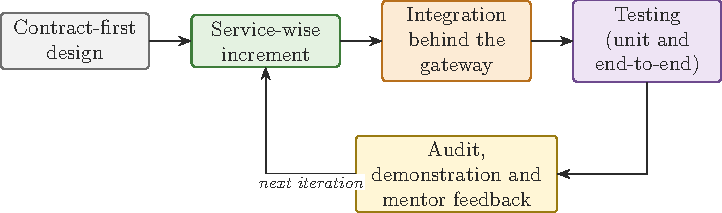
\includegraphics{figures/diagrams/sdlc}
\caption{Iterative and incremental development cycle}\label{fig:sdlc}
\end{figure}

\subsection{Requirement Analysis}
The requirements are grouped into functional requirements, which describe what the system does, and non-functional requirements, which describe the qualities and constraints it must satisfy. Every threshold mentioned below is a business rule that an administrator can change at run time; the values given are the current settings.

\subsubsection{Functional Requirements}
Table~\ref{tab:fr} lists the functional requirements and the agent responsible for each.

{\tablestyle
\begin{longtable}{|L{0.07\textwidth}|L{0.64\textwidth}|L{0.17\textwidth}|}
\caption{Functional requirements}\label{tab:fr}\\
\hline
\textbf{ID} & \textbf{Requirement} & \textbf{Agent} \\ \hline
\endfirsthead
\multicolumn{3}{l}{\small\textit{Table \thetable\ (continued)}}\\ \hline
\textbf{ID} & \textbf{Requirement} & \textbf{Agent} \\ \hline
\endhead
FR1 & Users can sign up, confirm their e-mail address, sign in and receive a 15-minute access token and a refresh token that logout revokes. Every endpoint checks the token and the role, except the health and metrics endpoints and the HMAC-authenticated signature webhooks. & Platform \\ \hline
FR2 & An administrator can view and edit the business rules (spend tiers, SLA, thresholds and tolerances); each change is versioned and reaches every service without a restart. & Platform \\ \hline
FR3 & Documents can be uploaded, e-mailed to an intake address or dropped into a watched folder. Each file is size- and type-checked and scanned for malware before storage; it is rejected if the scanner is unavailable. & Document and Vendor \\ \hline
FR4 & Documents are classified as invoice, purchase order, quotation or other; vendor, document number, date, currency, totals and line items are extracted. & Document and Vendor \\ \hline
FR5 & Each extracted field receives a confidence score. Documents below the threshold (0.8) go to a review queue, where fields can be corrected or confirmed. & Document and Vendor \\ \hline
FR6 & Vendors are matched by normalised name (fuzzy threshold 88); onboarding validates GSTIN format and check digit and IFSC codes and flags possible impostors. & Document and Vendor \\ \hline
FR7 & New or changed bank details stay pending, with payment held, until verified by a different user with the finance or admin role. & Document and Vendor \\ \hline
FR8 & Likely duplicate invoices are flagged (same vendor, amount within 2\%, date within 7 days, document number at least 85\% similar). & Document and Vendor \\ \hline
FR9 & Purchase requests follow approval chains by spend tier (automatic up to \Rs 500, manager up to \Rs 5,000, manager and finance above) and an approval-authority matrix; nobody can approve their own request. & Approval and Inventory \\ \hline
FR10 & Each request's approval runs as a durable Temporal workflow with reminders at 50\% and 80\% of the SLA; after 48 hours the request escalates to the next approver, and a timeout at the last level rejects it. Approvers can also decide from a single-use e-mail link for amounts up to \Rs 50,000. & Approval and Inventory \\ \hline
FR11 & Stock is reserved under a Redis lock so that concurrent requests cannot reserve the same unit; a request for out-of-stock items is back-ordered, and reorder suggestions are computed. & Approval and Inventory \\ \hline
FR12 & Licence usage is scored by an anomaly-detection model with per-licence explanations; an anomalous licence receives a reclaim request that waits through a seven-day grace period before approval. & Approval and Inventory \\ \hline
FR13 & Invoices are matched line by line against the purchase request, and an invoice exceeding the price or remaining balance by more than 1\% is held. & Approval and Inventory \\ \hline
FR14 & Contracts are generated from templates after approval and sent for signature automatically; renewal type, notice period and end date are extracted, and reminders are scheduled 60, 30 and 15 days before the notice deadline. & Contract and Risk \\ \hline
FR15 & Contracts are signed in the application with consent and a sealed audit record; signing for a vendor that is not cleared (High, provisional or unscored) requires an acknowledgement. External signature callbacks are accepted only with a valid HMAC signature and only once. & Contract and Risk \\ \hline
FR16 & Vendor risk is an integer score out of 100 from a deterministic ruleset, with a Low, Medium or High band and a rating status (assessed, provisional or not rated); a vendor with incomplete checks is never shown as Low, and a cancelled GSTIN, an invalid bank route or a potential sanctions match forces High until it is resolved. & Contract and Risk \\ \hline
FR17 & A clearance check states whether a vendor may be used for activation, a purchase or a contract; post-score decisions (approve, approve with conditions, accept risk, reject), evidence and disputes are recorded, and every score can be replayed exactly. & Contract and Risk \\ \hline
FR18 & Vendor offboarding revokes the vendor's access, flags active contracts for review and sets a data-retention flag instead of deleting records. & Contract and Risk \\ \hline
FR19 & The notification service consumes events, sends templated e-mail, sends urgent items immediately and batches routine ones into digests, retries failures and keeps a searchable log. & Platform \\ \hline
FR20 & An assistant answers questions from the platform's own contracts, documents, rules and records by retrieval-augmented generation, cites its sources, says when it cannot find an answer, and retrieves only what the asking user may see. & Platform \\ \hline
FR21 & The frontend provides role-specific navigation and dashboards, a request wizard, an approval inbox, one home page per request, document, vendor, licence and contract, and pages for notifications, spend analysis, business rules, users, audit activity, system health and the Kafka event log. & Frontend \\ \hline
FR22 & Significant actions on documents, vendors, requests and contracts are written to an audit log that administrators can query. & All \\ \hline
FR23 & Each request is checked against its department's budget for the category and fiscal quarter; a request that would exceed it receives a finance approval step, and concurrent requests cannot both use the last amount. & Approval and Inventory \\ \hline
FR24 & Obligations are read from signed contracts and confirmed by finance; confirmed obligations are reminded before their due date, recorded downtime yields the contractual service credit, and a licence with more users than the contract allows is flagged. & Contract and Risk \\ \hline
FR25 & Requesters order from an IT catalog whose agreed prices, vendor and type override client input; expired items cannot be ordered, and a received seat add-on increases the licence's seats. & Approval and Inventory \\ \hline
FR26 & Finance runs request-for-quotation events with sealed quotes, quotes linked from the document pipeline by reference, weighted comparison, further rounds and an award that creates the purchase request. & Approval and Inventory \\ \hline
FR27 & Deliveries are recorded per line with asset tags; invoices may not exceed the quantity received; each vendor has a performance scorecard. & Approval and Inventory, Contract and Risk \\ \hline
FR28 & Every invoice is checked for GST (GSTIN, tax split, rate per HSN or SAC code, totals, e-invoice QR signature); a failed check forces review without changing the confidence score. TDS is computed at booking, the GSTR-2B statement is reconciled, and MSME payment deadlines are tracked. & Document and Vendor, Approval and Inventory \\ \hline
\end{longtable}}

\subsubsection{Non-Functional Requirements}
Table~\ref{tab:nfr} lists the qualities and constraints the system must satisfy.

\begin{table}[!htbp]
\centering\tablestyle
\caption{Non-functional requirements}\label{tab:nfr}
\begin{tabularx}{\textwidth}{|L{0.18\textwidth}|Y|}
\hline
\textbf{Category} & \textbf{Requirement} \\ \hline
Security & JWT authentication and role checks in every service; identity taken only from the token; argon2id password hashing and breached-password check; account lockout and gateway rate limits; fail-closed malware scanning; HMAC-verified webhooks; dual control of payment details; per-service Kafka credentials and topic permissions; only the gateway port exposed. \\ \hline
Reliability & Approval, reclaim and renewal workflows are durable (Temporal). Events are published through a transactional outbox; consumers are idempotent, retry and dead-letter failures; a sweep re-queues stranded documents; a timed-out last approval is rejected, never approved by default. \\ \hline
Consistency & A common REST envelope and error format; a purchase-request state machine enforced in code and by a database constraint; idempotent migrations owned by each service. \\ \hline
Performance & Uploads return once the file is stored; reading, OCR and model inference run in background workers with time limits. \\ \hline
Traceability & Every event carries an event ID, source and correlation ID; logs from every service are collected centrally and searchable by correlation ID; significant actions are audited; model-routing decisions are logged. \\ \hline
Explainability & Confidence scores per field, risk factors per vendor, SHAP reasons per licence and the risk shown before signing. \\ \hline
Maintainability & Responsibilities separated by service; shared contracts documented; thresholds held as business rules, each with a behaviour test. \\ \hline
Portability & The stack is containerised and runs on macOS, Linux and Windows through WSL2. \\ \hline
\end{tabularx}
\end{table}

\noindent\textbf{Constraints and assumptions.} Payment execution, ERP integration, a third-party e-signature provider and automatic model retraining are outside the scope. GST and TDS rates are seeded values that a chartered accountant must confirm. Kafka traffic is authenticated but not encrypted, which is acceptable only on a single host. The vendor risk data, licence usage logs, classifier corpus and sample documents are synthetic.

\subsection{UML Diagrams and Data Flow Diagrams}

\subsubsection{Use Case Diagram}
The use case diagram is shown in Figure~\ref{fig:usecase} in Chapter~\ref{chap3}. It identifies the Requester, Approver, Finance user and Administrator and groups their activities into authentication and rules, purchase and inventory, vendor intelligence, contract and risk, and notification.

\subsubsection{Data Flow Diagram -- Level 0}
The context diagram (Figure~\ref{fig:dfd0}) shows the platform as a single process and its exchanges with the external entities: the three groups of users, vendors who send documents, the e-mail service, and the external lookup services.

\begin{figure}[!htbp]
\centering
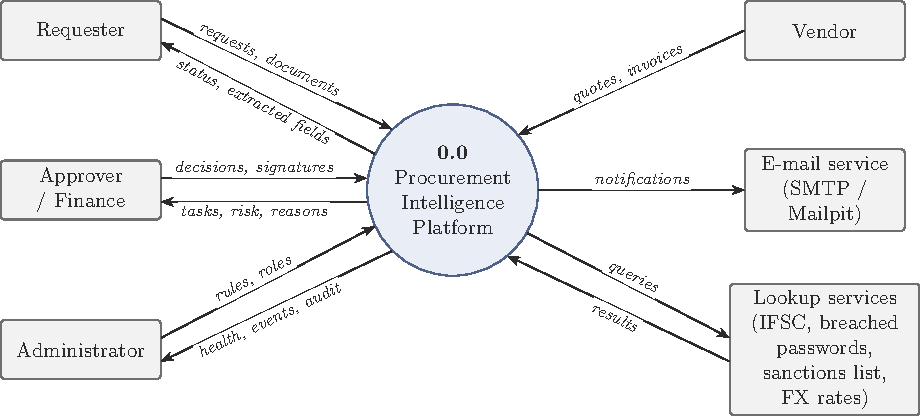
\includegraphics{figures/diagrams/dfd0}
\caption{Level 0 data flow diagram (context diagram)}\label{fig:dfd0}
\end{figure}

\subsubsection{Data Flow Diagram -- Level 1}
The Level 1 diagram (Figure~\ref{fig:dfd1}) decomposes the platform into the processes of Table~\ref{tab:dfd}. Processes 2.0 to 5.0 exchange events through the messaging layer, process 6.0 consumes them, and process 1.0 issues the tokens and rules that the others check.

\begin{figure}[!htbp]
\centering
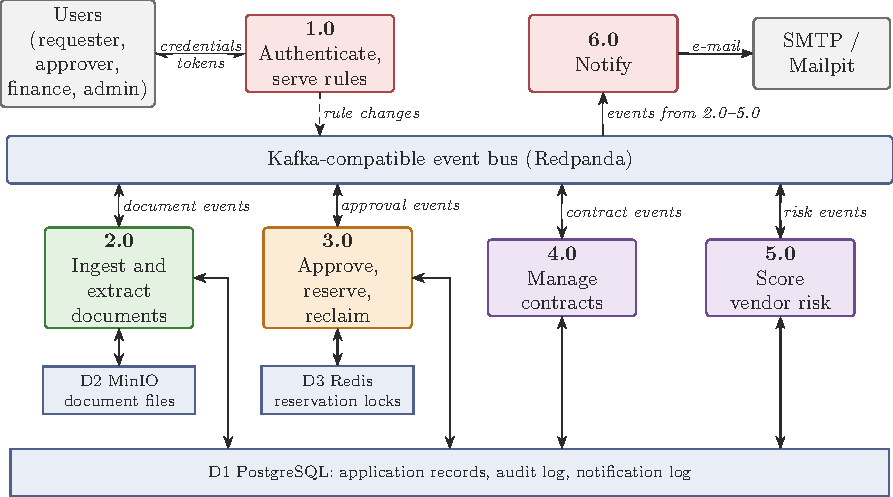
\includegraphics{figures/diagrams/dfd1}
\caption{Level 1 data flow diagram}\label{fig:dfd1}
\end{figure}

\begin{table}[!htbp]
\centering\tablestyle
\caption{Level 1 DFD processes}\label{tab:dfd}
\begin{tabularx}{\textwidth}{|C{0.09\textwidth}|L{0.18\textwidth}|L{0.26\textwidth}|Y|}
\hline
\textbf{Process} & \textbf{Name} & \textbf{Inputs} & \textbf{Outputs} \\ \hline
1.0 & Authenticate, serve rules & Credentials, refresh token, rule edits & Access and refresh tokens, role, rule changes \\ \hline
2.0 & Ingest and extract documents & Uploaded, e-mailed or dropped file & Classified document, vendor match, review-queue items, invoice match \\ \hline
3.0 & Approve, reserve, reclaim & Purchase request, decisions, usage logs & Decisions, reservations, escalations, reclaim requests \\ \hline
4.0 & Manage contracts & Approved request, signature & Contract text and PDF, signature record, renewal reminders \\ \hline
5.0 & Score vendor risk & Vendor signals, sanctions list & Points per check, band, rating status, overrides, clearance \\ \hline
6.0 & Notify & Events from 2.0--5.0 & E-mail, digests, notification log \\ \hline
\end{tabularx}
\end{table}

\subsubsection{Sequence Diagram}
Figure~\ref{fig:sequence} follows one purchase request from creation to signature. It shows the synchronous calls through the gateway, the asynchronous events, and the point at which the Temporal workflow hands the decision back to the service.

\begin{figure}[!htbp]
\centering
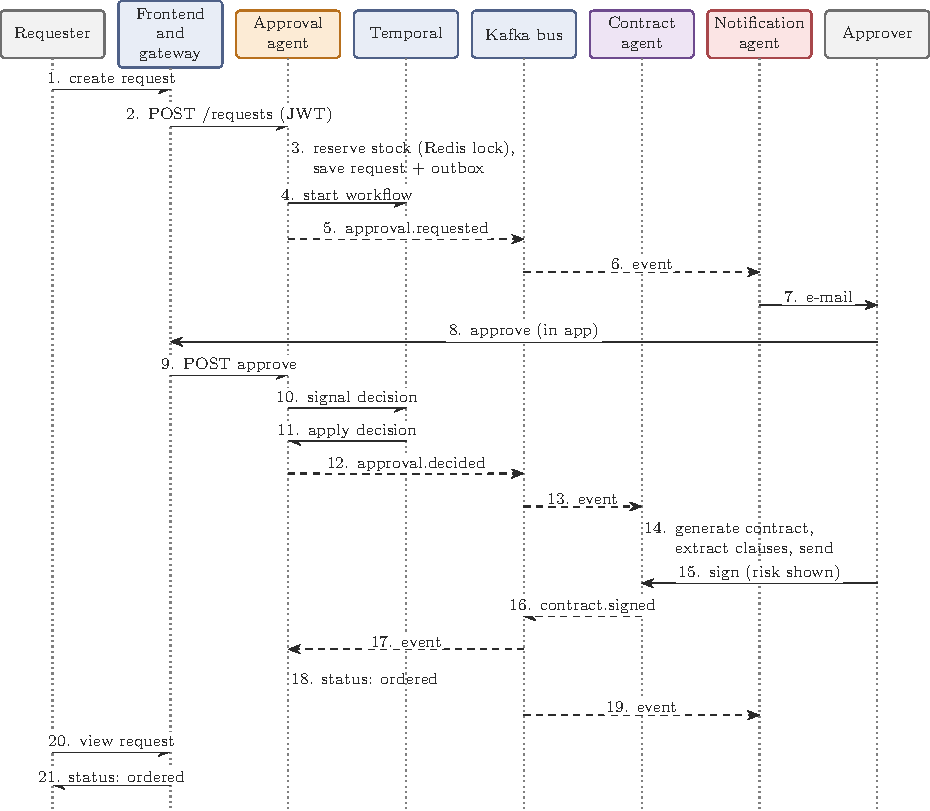
\includegraphics{figures/diagrams/sequence}
\caption[Sequence diagram of the purchase-request journey]{Sequence diagram of the purchase-request journey (solid: synchronous call; dashed: asynchronous event)}\label{fig:sequence}
\end{figure}

\subsubsection{Activity Diagram: Document Processing}
The activity diagram (Figure~\ref{fig:activity}) shows the decisions taken for one document. The upload is rejected if the file fails a check, is infected or cannot be scanned; a file that cannot be read fails with a message for the uploader. A readable file is classified, extracted, matched and scored. A document meeting the threshold, with no rule forcing review, is completed; otherwise it waits in the review queue until a reviewer corrects or confirms it.

\begin{figure}[!htbp]
\centering
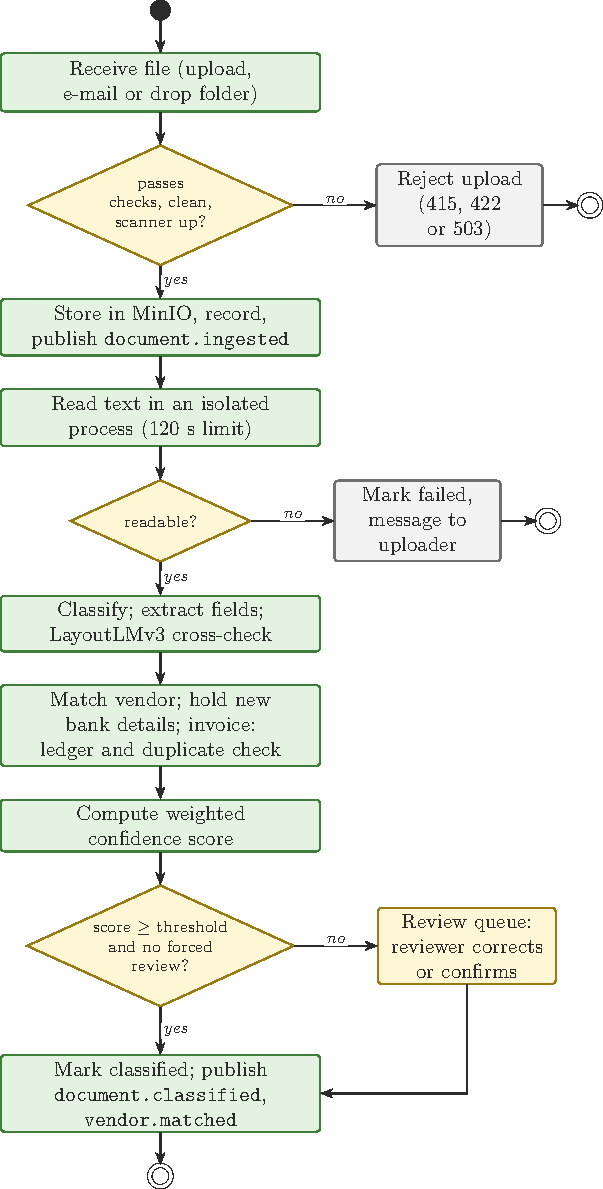
\includegraphics{figures/diagrams/activity}
\caption{Activity diagram of document processing}\label{fig:activity}
\end{figure}

\subsubsection{Purchase-Request State Machine}
A purchase request moves through the states of Figure~\ref{fig:states}. The allowed transitions are defined once in a shared module and checked on every status change, and the database rejects any status outside the list. An event that arrives after the request has already moved past the state it would cause (for example a late \code{contract.signed}) is recognised and ignored rather than treated as an error.

\begin{figure}[!htbp]
\centering
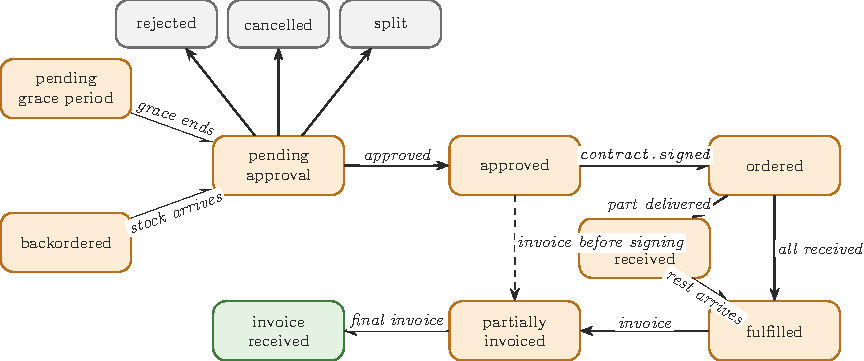
\includegraphics{figures/diagrams/states}
\caption[State machine of a purchase request]{State machine of a purchase request (main transitions; stored state names use underscores, for example \code{pending_approval}; a request can also be cancelled from the waiting states)}\label{fig:states}
\end{figure}

\subsubsection{Entity Relationship Diagram}
All services share one PostgreSQL database of about fifty tables; each service creates and migrates its own. Figure~\ref{fig:er} shows the main entities and their foreign keys as they exist in the running database. The vendor is the central entity: documents, purchase requests, contracts, licences, risk scores, sanctions screenings and payment-change requests all refer to it. The \code{inventory} table has no foreign key: requests refer to stock by SKU inside their items. The extensions of Section~\ref{sec:extensions} add \code{budgets}, \code{contract_obligations}, \code{obligation_events}, \code{sla_credits}, \code{catalog_items}, \code{rfq_events}, \code{rfq_invitations}, \code{rfq_responses}, \code{goods_receipts}, \code{vendor_scorecards}, \code{gst_rates}, \code{gstr2b_uploads} and \code{tds_sections}, and the deterministic risk scorecard adds \code{risk_rulesets}, \code{risk_score_rule_results}, \code{vendor_signal_observations}, \code{vendor_signal_raw_responses}, \code{vendor_evidence}, \code{vendor_assessment_disputes} and \code{vendor_decisions} (scores and observations are append-only); each refers to a request, contract, licence or vendor of the figure. Supporting tables, not shown, hold users and tokens, business rules and their history, the event outbox, inbox and dead-letter table, the Kafka event log, notification and model-routing logs, the reviewer-feedback tables, and the assistant's chat sessions and \code{document_embeddings} index (one row per passage, with its 768-dimensional vector, source, section and audience).

\begin{figure}[!htbp]
\centering
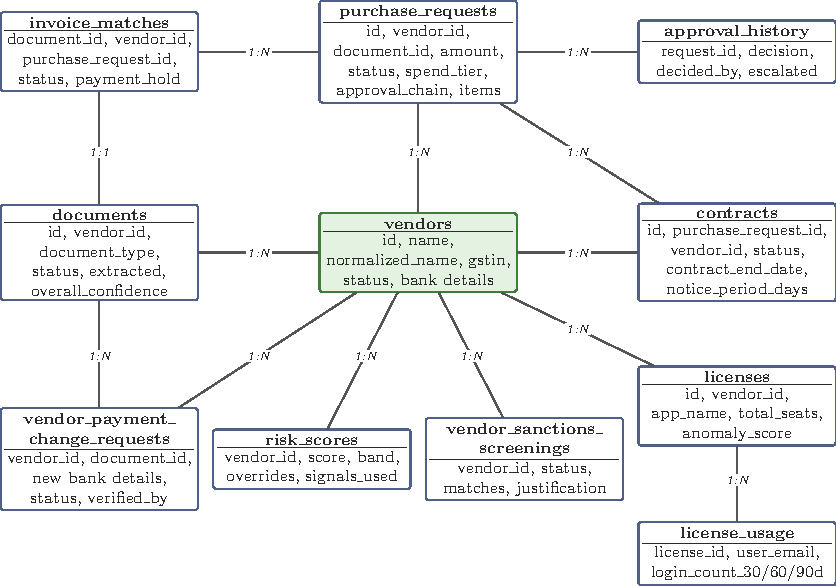
\includegraphics{figures/diagrams/er}
\caption[Entity relationship diagram of the main entities]{Entity relationship diagram of the main entities (foreign keys as in the running database; \code{invoice_matches} also refers to \code{vendors})}\label{fig:er}
\end{figure}

\subsection{Cost Analysis}
The project uses only open-source software and free API tiers, so it incurs no software-licence cost, and it was developed on the team's own laptops. The potential costs are team effort, paid API tiers if live registry lookups are enabled, cloud hosting, and a production e-mail service. The estimates in Table~\ref{tab:cost} are indicative and should be revised against real quotations.

\begin{table}[!htbp]
\centering\tablestyle
\caption{Indicative cost analysis}\label{tab:cost}
\begin{tabularx}{\textwidth}{|L{0.18\textwidth}|Y|L{0.20\textwidth}|}
\hline
\textbf{Item} & \textbf{Basis} & \textbf{Indicative cost} \\ \hline
Software licences & Python, FastAPI, PostgreSQL, Redis, Redpanda, MinIO, Temporal, MLflow, Prometheus, Grafana, Loki, ClamAV, Docling, PaddleOCR, Hugging Face models, Ollama, React and Docker are open source & \Rs 0 \\ \hline
Development hardware & Existing student laptops & \Rs 0 additional \\ \hline
External APIs & HaveIBeenPwned range API, IFSC directory and Frankfurter exchange rates are free; the OpenSanctions list is free for non-commercial use only (CC BY-NC 4.0) and needs a licence for commercial use; live GSTIN lookups depend on the provider's quota & \Rs 0 in the project; depends on usage and licensing in production \\ \hline
Team effort & Part-time project work by four students & Not monetised \\ \hline
Optional cloud hosting & One virtual machine with about 4--8 vCPU and 16\,GB RAM, plus storage and backups & Approx.\ \Rs 6,000--10,000 per month \\ \hline
E-mail delivery & Production SMTP service instead of the development mail catcher & A few hundred rupees per month at pilot volume \\ \hline
\end{tabularx}
\end{table}

A meaningful break-even estimate needs measured document volumes, licence costs and the time saved or duplicate payments avoided. Those figures are not available, so no return-on-investment claim is made.

\subsection{Hardware and Software Requirements}
The stack runs 24 containers on one Docker host. Measured on 16 October 2026, it used about 3.2\,GB of RAM when idle and more while reading scanned documents, and its images occupied about 15\,GB before build cache and data volumes. ClamAV alone needs about 1\,GB of memory. Table~\ref{tab:hw} gives the resulting requirements and Table~\ref{tab:sw} the software.

\begin{table}[!htbp]
\centering\tablestyle
\caption{Hardware requirements}\label{tab:hw}
\begin{tabularx}{\textwidth}{|L{0.16\textwidth}|L{0.34\textwidth}|Y|}
\hline
\textbf{Component} & \textbf{Minimum} & \textbf{Recommended} \\ \hline
Processor & 4 cores & 8 cores \\ \hline
Memory & 8\,GB available to Docker & 16\,GB RAM \\ \hline
Storage & 40\,GB free & 80\,GB free for images, models (about 1\,GB), sanctions data and volumes \\ \hline
Network & Required for the first build, model and sanctions downloads, and sign-up's breached-password check & Broadband connection \\ \hline
GPU & Not required & Optional, for faster OCR and transformer inference \\ \hline
\end{tabularx}
\end{table}

\begin{table}[!htbp]
\centering\tablestyle
\caption{Software requirements}\label{tab:sw}
\begin{tabularx}{\textwidth}{|L{0.20\textwidth}|Y|}
\hline
\textbf{Category} & \textbf{Requirement} \\ \hline
Operating system & macOS, Ubuntu/Linux, or Windows 10/11 with WSL2 \\ \hline
Container runtime & Docker Engine or Docker Desktop with Compose v2 \\ \hline
Backend & Python 3.11, FastAPI, SQLAlchemy, Alembic, pytest, scikit-learn, SHAP, Transformers, rapidfuzz, Jinja2 \\ \hline
Frontend & React, TypeScript, Vite and Tailwind CSS, built in a Node 20 container \\ \hline
Data and messaging & PostgreSQL, Redis, Redpanda (Kafka API) and MinIO \\ \hline
Workflow and ML & Temporal, MLflow \\ \hline
Document processing & pdfplumber, Docling, PaddleOCR, LayoutLMv3 (optional download), ClamAV \\ \hline
Monitoring and mail & Prometheus, Grafana, Loki, Promtail, kafka-exporter, Mailpit \\ \hline
Assistant & Ollama on the host with Llama 3.2 (3B) and nomic-embed-text; PostgreSQL with pgvector \\ \hline
Gateway and browser & Nginx; a current Chrome, Edge, Firefox or Safari \\ \hline
\end{tabularx}
\end{table}

\section{System Architecture}
The platform follows a modular, event-driven architecture in which independent services each own one procurement function. The frontend talks to the services through the gateway with synchronous HTTP requests where an immediate answer is needed, while the services talk to one another mainly through events. Temporal runs the long-lived workflows; PostgreSQL holds the records, Redis the locks and caches, and MinIO the files. Background workers consume events and run slow tasks, so users get a response without waiting for every downstream step.

\subsection{UI/UX Design}
The frontend is a React and TypeScript single-page application built with Vite and Tailwind CSS. Nginx serves it and routes its API calls, so the page and the API share one origin. The interface follows these principles:
\begin{enumerate}
  \item \textbf{Role-aware navigation:} each role sees its own navigation and dashboard. Frontend route checks are only for usability; every endpoint enforces authorisation itself.
  \item \textbf{One home page per item:} a request, document, vendor, licence and contract each have one page where all their actions live; lists, dashboards and the approval inbox link to it. A request page shows a clickable lifecycle whose steps open their details and actions.
  \item \textbf{Clear asynchronous status:} decisions and document processing complete in background workers, so the interface polls briefly after an action and shows each step as it settles; a step is shown as in progress only while an agent is actually working on it.
  \item \textbf{Human review:} extracted fields are shown with their confidence and can be corrected or confirmed; risk factors, licence anomaly reasons and the vendor's risk at signing are always visible.
  \item \textbf{Honest limits:} where a feature has no backend support the interface shows it as unavailable rather than pretending it succeeded.
  \item \textbf{Demonstration support:} the sign-in page offers one-click demo accounts in development builds, and a command palette (Ctrl/Cmd+K) searches loaded requests, vendors, contracts and documents.
\end{enumerate}
Screenshots of the implemented screens are given in Section~\ref{sec:screens}, and Table~\ref{tab:screens} lists the principal screens.

\begin{table}[!htbp]
\centering\tablestyle
\caption{Principal screens and their purposes}\label{tab:screens}
\begin{tabularx}{\textwidth}{|L{0.22\textwidth}|L{0.20\textwidth}|Y|}
\hline
\textbf{Screen} & \textbf{User role} & \textbf{Purpose} \\ \hline
Sign in, sign up, password reset & All & Account access and e-mail verification \\ \hline
Dashboards & Each role & Own requests, items awaiting approval, spend overview or system overview \\ \hline
New request wizard & Requester & Enter details, choose a vendor, optionally upload a document with live pipeline status, review extracted fields and submit \\ \hline
Request page & All, by permission & Clickable lifecycle, approval, procurement checks (budget, sourcing), deliveries, invoice ledger, contract and signature \\ \hline
Approval inbox & Approver, finance & Pending requests and reclaims for the levels assigned to the user, with SLA status \\ \hline
Document page & Requester, approver, finance, admin & Preview, extracted fields with confidence, correction and confirmation \\ \hline
Vendor page and onboarding & Finance, admin & Risk scorecard with points per check, performance scorecard, bank-detail verification, sanctions status, onboarding checks \\ \hline
Licence page & Approver, finance, admin & Usage trend, anomaly score and reasons, contract seat limit, open reclaim request \\ \hline
Contract page & Approver, finance, admin & Contract text, renewal dates, signing dialog, signed copy and certificate; obligations with confirmation, downtime and service credits \\ \hline
Budgets & Approver, finance, admin & Budgets per department, category and quarter with consumed, committed, pending and remaining amounts \\ \hline
IT catalog & All (editing: finance, admin) & Order approved items at agreed prices; add, reprice or switch off items \\ \hline
Sourcing & Approver, finance, admin & RFQ list and RFQ page: invitations, sealed or open quotes, weighted comparison, rounds and award \\ \hline
GST & Approver, finance, admin & Month figures, GST check of each invoice, GSTR-2B reconciliation, MSME deadlines, TDS register and rate tables \\ \hline
Inventory, spend analysis, risk & Finance, admin & Stock and reorder suggestions, spend by category, vendor risk bands and weekly scorecard monitoring \\ \hline
Business rules, users & Admin & Edit rules with history; manage roles \\ \hline
Control Panel, Controls, System Health, Audit & Admin (Controls: finance too) & Kafka event log and failed events, platform controls, service and model-routing status, audit trail \\ \hline
Notifications, account & All & Notification history; password change and sign-out everywhere \\ \hline
Assistant drawer & All & Questions in plain language, answered from the contracts, documents, rules and records the user may see, with cited references \\ \hline
\end{tabularx}
\end{table}

\subsection{Block Diagram}
The block diagram (Figure~\ref{fig:block}) shows the deployed components and their connections on the single Docker host. Table~\ref{tab:layers} describes each layer.

\begin{figure}[!htbp]
\centering
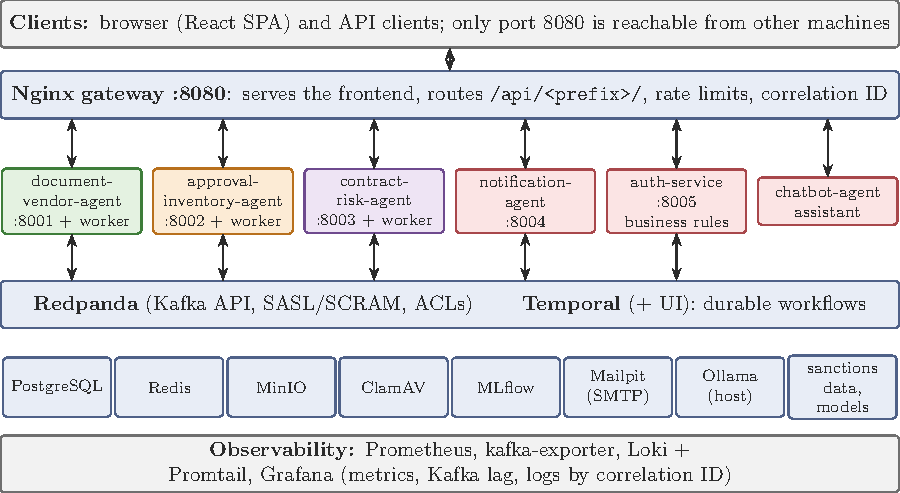
\includegraphics{figures/diagrams/block}
\caption{Block diagram of the deployed system}\label{fig:block}
\end{figure}

\begin{table}[!htbp]
\centering\tablestyle
\caption{Architectural layers}\label{tab:layers}
\begin{tabularx}{\textwidth}{|L{0.19\textwidth}|Y|}
\hline
\textbf{Layer} & \textbf{Components and responsibilities} \\ \hline
Clients & The React application and API clients reach the platform only through the gateway on port 8080. \\ \hline
Gateway & Nginx serves the frontend, routes API paths to the services, limits request rates on authentication endpoints and assigns a correlation ID. \\ \hline
Application services & Document and Vendor agent (8001), Approval and Inventory agent (8002), Contract and Risk agent (8003), notification agent (8004), authentication and business-rules service (8005) and the assistant. Every service checks the JWT and role, except health, metrics and the HMAC-signed webhooks. \\ \hline
Background workers & The document, approval and contract services each run a worker that consumes events, runs Temporal workflows and performs slow tasks such as OCR and model inference. \\ \hline
Messaging and orchestration & Redpanda carries the events with per-service credentials; Temporal runs the approval, reclaim and renewal workflows. \\ \hline
Data and platform services & PostgreSQL holds the records, Redis the reservation locks and rule caches, and MinIO the files. ClamAV scans uploads, MLflow tracks the trained models, Mailpit receives development e-mail, and Ollama runs the assistant's model on the host. \\ \hline
Observability & Prometheus collects metrics, Loki collects logs, and Grafana shows request rates, latency, errors, Kafka consumer lag and the logs of one correlation ID across services. \\ \hline
\end{tabularx}
\end{table}

\subsection{Main Data Paths}
The principal data paths are:
\begin{enumerate}
  \item \textbf{User access:} the browser loads the frontend from Nginx; API calls are routed to the right service after the gateway strips the \texttt{/api/<prefix>/} segment.
  \item \textbf{Document processing:} the Document and Vendor agent checks and scans an upload, stores it in MinIO and publishes \code{document.ingested} through the outbox. Its worker reads, classifies and extracts the document and publishes \code{document.classified} and \code{vendor.matched}.
  \item \textbf{Approval processing:} the Approval and Inventory agent reserves stock, saves the request and starts a Temporal workflow. An approve or reject call signals the workflow; the worker applies the decision, updates the status and publishes \code{approval.decided}.
  \item \textbf{Contract processing:} the Contract and Risk agent generates the contract for an approved request and sends it for signature. When it is signed, \code{contract.signed} moves the request to \emph{ordered}; marking the goods as received makes it \emph{fulfilled}, and the vendor's invoice is matched against it.
  \item \textbf{Risk assessment and notifications:} the Contract and Risk agent publishes risk, renewal and offboarding events; the notification agent consumes them and sends e-mail.
  \item \textbf{Supporting services:} PostgreSQL stores the records (with pgvector for the assistant's index), Redis guards reservations, MinIO stores files, and MLflow records the training runs of the trained models.
\end{enumerate}
Together, these paths show how synchronous API calls, asynchronous events and durable workflows combine to carry a request from intake to completion.
